\chapter{Experiments Conducted}\label{chap:exp}

In this chapter, we outline all experiments conducted and discuss the results.
\todoA{az to bude hotove}

Since the objective of this thesis is to compare several approaches,
next step after building the architecture was to define sets of experiments and metrics to compare the results.
Our original intention was to try all combinations of features, classifiers and other techniques.
However, this turned out to be computationally infeasible.
Instead, we tried promising subsets by only choosing the best variant out of each group and combine it.

The training and testing was done on a dataset with 64,550 instances.
For each evaluation, 10-fold crossvalidation was used, resulting in
training sets with 58,095 instances and testing with 6,455 instances.

For labels, we used the number of useful likes.
Reviews with zero likes were labelled not-useful and
reviews with at least two likes useful.
1 like reviews were dropped.
The entire dataset contains 44,921 not-useful and
19,629 useful instances.

We split features into the sets defined in the two lists bellow.
The first list contains existential features --- they express that certain phrase is present in the review.

\begin{itemize}
	\item UNIGRAMS --- top 50,000 unigrams according to mutual information
	\item BIGRAMS --- bigrams consisting of top 25,000 adjacent unigrams
	\item TRIGRAMS  --- trigrams consisting of top 10,000 adjacent unigrams
	\item TFIDF  --- top 50,000 words
	\item ENTITIES --- 270,000 entities as found by the NLP analysis
\end{itemize}

Note that the best way for selecting bigrams and trigrams would be to compute mutual information of all bigrams, resp. trigrams.
However, this is computationally very expensive, as there is well over 1,100,000 unique bigrams in the reviews.
Instead, we decided to use n-grams that consist of top unigrams only as described in the list.

The threshold of n-grams and TF-IDF were found experimentally to produce approximately the same number of features as entities.
\todoA{not true}

The second list contains threshold features --- they split reviews into groups based on some property reaching a threshold.

\begin{itemize}
	\item STARS 
		\begin{itemize}
			\item the number of stars; five groups
			\item indicators for each stars number; five pairs one-vs-rest
			\item extreme stars; one group 1 or 5 stars; the rest another group
			\item the number of average stars for the business; five groups
		\end{itemize}
	\item REVIEWLEN 
		\begin{itemize}
			\item the number of words; three groups with thresholds 50 and 150
			\item the number of words; five pairs with thresholds 35, 50, 75, 100 and 150
		\end{itemize}
	\item SPELLCHECK 
		\begin{itemize}
			\item the rate of misspelled words; five pairs with thresholds 0.02, 0.05, 0.1, 0.15 and 0.2
			\item the number of misspelled words; four pairs with thresholds 5, 10, 15 and 20
		\end{itemize}
	
	\item COSINESIM --- cosine similarity to 10 randomly chosen useful instances; five pairs with thresholds 0.4, 0.6, 0.8, 0.9, 0.95
\end{itemize}

We performed the analysis in five rounds.
We report f-measure and accuracy of all models to retain comparability even throughout rounds.
Each round focuses on a different variable as listed bellow:

\begin{enumerate}
	\item baseline; (plus compute mutual information)
	\item feature sets with Na\"{\i}ve Bayes
	\item feature selection algorithms
	\item classifiers
	\item size of training data
\end{enumerate}


\section{1st round --- Baseline}

In this round, we ran zero-R and one-R to get an idea about the problem.
Also, we computed mutual information of all features.

Zero-R achieves accuracy of 70\% as reported in \Cref{tab:base_perf}.
This is in compliance with the label distribution,
because the dataset contains approximately the same proportion of not-useful instances.
One-R raises this performance a bit to 73\%.

Because zero-R assigns all instances label \textit{not-useful},
there are no true positive instances.
Hence precision and recall are zero.
For this reason, f-measure is undefined for zero-R.
For f-measure, we use the baseline performance of one-R --- 56\%.

\begin{table}[h!]

\centering
\begin{tabular}{lr@{~}r@{~}rr@{~}r@{~}r}
\toprule
\textbf{name}	& \multicolumn{3}{c}{\textbf{f-measure}} & \multicolumn{3}{c}{\textbf{accuracy}} \\
\midrule
zero-R & \multicolumn{3}{c}{N/A} & 0.70 & (0.69, 0.70) & $\pm$ 0.004 \\
one-R & 0.56 & (0.54, 0.58) & $\pm$ 0.012 & 0.73 & (0.72, 0.74) & $\pm$ 0.005 \\

\bottomrule
\end{tabular}

\caption{Performance of Feature Selections}\label{tab:base_perf}
All reported values are in the format `value (min, max) $\pm$ standard deviation'.
\end{table}

\section{2nd round --- Features}

In this round, we run Na\"{\i}ve Bayes with different sets of features.
Configurations with results are shown in \Cref{tab:feat_perf}.
Names refer to feature sets.
\textbf{\{uni,bi\}grams} and \textbf{\{uni,bi,tri\}grams} are listed n-grams together.
\textbf{basic} is STARS, REVIEWLEN, SPELLCHECK and COSINESIM.

We can clearly see that none of the feature set brought desired improvement.
Only feature set \textbf{basic} brought a 3 percent improvement in f-measure.
Other sets brought immense deterioration.
Any combination of \textbf{Bigrams} or \textbf{TF-IDF} decreased the accuracy by at least 30\%.
This is probably due to overfitting.
The feature sets contains so many features, that our model learnt to recognise
irregularities in the data.
This claim supports a brief analysis of the features showing that
even words like `in', `to' or `that,' which clearly carry no information about usefulness.
It is interesting to note that f-measure did not suffer from such a big decrease.



\begin{table}[h!]

\centering
\begin{tabular}{lr@{~}r@{~}rr@{~}r@{~}r}
\toprule
\textbf{name}	& \multicolumn{3}{c}{\textbf{f-measure}} & \multicolumn{3}{c}{\textbf{accuracy}} \\
\midrule
unigrams& 0.47 & (0.46, 0.48) & $\pm$ 0.007 & 0.30 & (0.29, 0.32) & $\pm$ 0.006 \\
tfidf& 0.47 & (0.46, 0.48) & $\pm$ 0.007 & 0.30 & (0.29, 0.32) & $\pm$ 0.006 \\
\{uni,bi\}grams	& 0.47 & (0.46, 0.47) & $\pm$ 0.005 & 0.30 & (0.30, 0.31) & $\pm$ 0.004\\
bigrams & 0.47 & (0.46, 0.47) & $\pm$ 0.005 & 0.31 & (0.30, 0.31) & $\pm$ 0.005			\\
entities & 0.48 & (0.47, 0.49) & $\pm$ 0.005 & 0.35 & (0.34, 0.36) & $\pm$ 0.005		\\
\{uni,bi,tri\}grams & 0.47 & (0.46, 0.48) & $\pm$ 0.008 & 0.30 & (0.29, 0.32) & $\pm$ 0.007	\\
trigrams & 0.47 & (0.46, 0.49) & $\pm$ 0.008 & 0.32 & (0.31, 0.33) & $\pm$ 0.006		\\
cosine\_sim & \multicolumn{3}{c}{N/A} & 0.70 & (0.69, 0.70) & $\pm$ 0.006		\\
\textbf{basic} & 0.59 & (0.58, 0.60) & $\pm$ 0.005 & 0.71 & (0.71, 0.72) & $\pm$ 0.004		\\
basic+bigrams & 0.48 & (0.47, 0.49) & $\pm$ 0.007 & 0.35 & (0.34, 0.36) & $\pm$ 0.006		\\
basic+tfidf & 0.48 & (0.47, 0.50) & $\pm$ 0.007 & 0.36 & (0.35, 0.37) & $\pm$ 0.006			\\
\textbf{basic+entities} & 0.55 & (0.54, 0.56) & $\pm$ 0.008 & 0.54 & (0.53, 0.55) & $\pm$ 0.006		\\
\bottomrule
\end{tabular}


\caption{Performance of Feature Configurations}\label{tab:feat_perf}
All reported values are in the format `value (min, max) $\pm$ standard deviation'.
\end{table}


\section{3rd round --- Feature Selection}

In this round, we compare three different methods of feature selection.
The attempt is to avoid the overfitting described in the previous section.
We use features \textbf{basic+entities} and Na\"{i}ve Bayes.
We run PCA with 100 dimensions as recommended by scipy documentation.
For mutual information and chi square, we choose top 1000 features.

From \Cref{tab:sel_perf}, we can see that both mutual information
and chi-square improved the accuracy to 58\% and f-measure even to the original
0.56 from the baseline.
Choosing the threshold for the number of features more carefully could improve the results even further, possible above the performance of the baseline.
We have not analyzed this due the lack of time.

PCA decreased the performance by a significant margin.
This could be due to non-optimal parameters, which
again could be improved by more careful analysis.

\begin{table}[h!]

\centering
\begin{tabular}{lr@{~}r@{~}rr@{~}r@{~}r}
\toprule
\textbf{name}	& \multicolumn{3}{c}{\textbf{f-measure}} & \multicolumn{3}{c}{\textbf{accuracy}} \\

\midrule
basic+entities & 0.55 & (0.54, 0.56) & $\pm$ 0.008 & 0.54 & (0.53, 0.55) & $\pm$ 0.006		\\
\textbf{basic+entities[MI]} & 0.56 & (0.55, 0.57) & $\pm$ 0.007 & 0.58 & (0.57, 0.60) & $\pm$ 0.008 \\
\textbf{basic+entities[CHI]} & 0.56 & (0.55, 0.57) & $\pm$ 0.007 & 0.58 & (0.57, 0.59) & $\pm$ 0.007 \\
basic+entities[PCA] & 0.47 & (0.46, 0.48) & $\pm$ 0.007 & 0.30 & (0.3, 0.31) & $\pm$ 0.006 \\


\bottomrule
\end{tabular}

\caption{Performance of Feature Selections}\label{tab:sel_perf}
All reported values are in the format `value (min, max) $\pm$ standard deviation'.
\end{table}

\section{4th round --- Classifiers}

In the fourth round, we decided to try different classifiers as opposed the previously used Na\"{\i}ve Bayes.
For Na\"{\i}ve Bayes, we chose the best performing model with the only feature set \textbf{basic}.
FastText was used without any features, only with raw text.
Lastly, we used decision tree.
Decision tree tends to suffer from overfitting when too many features are used.
Also, the training time increases significantly with the number of features,
because mutual information needs to be computed for all features in all nodes.
Therefore, we used only feature set \textbf{basic}.

The results can be seen in \Cref{tab:clsf_perf}.
The performance of FastText was comparable to Na\"{\i}ve Bayes on \textbf{basic+entities}.
The best performance was achieved by decision tree.
It improves the previous top performing one-R by 3\%, but decreasing the f-measure.
This is a reasonable result, since one-R is a special simpler case of decision tree.


\begin{table}[h!]

\centering
\begin{tabular}{lr@{~}r@{~}rr@{~}r@{~}r}
\toprule
\textbf{name}	& \multicolumn{3}{c}{\textbf{f-measure}} & \multicolumn{3}{c}{\textbf{accuracy}} \\
\midrule

Na\"{\i}ve Bayes & 0.59 & (0.58, 0.60) & $\pm$ 0.005 & 0.71 & (0.71, 0.72) & $\pm$ 0.004		\\

FastText & 0.53 & (0.52, 0.54) & $\pm$ 0.009 & 0.55 & (0.54, 0.57) & $\pm$ 0.008 \\
\textbf{Decision tree} & 0.52 & (0.49, 0.54) & $\pm$ 0.012 & 0.74 & (0.73, 0.74) & $\pm$ 0.004 \\

\bottomrule
\end{tabular}

\caption{Performance of Different Classifiers}\label{tab:clsf_perf}
All reported values are in the format `value (min, max) $\pm$ standard deviation'.
\end{table}


\section{5th round --- Training Size}

\begin{figure}[h]\centering
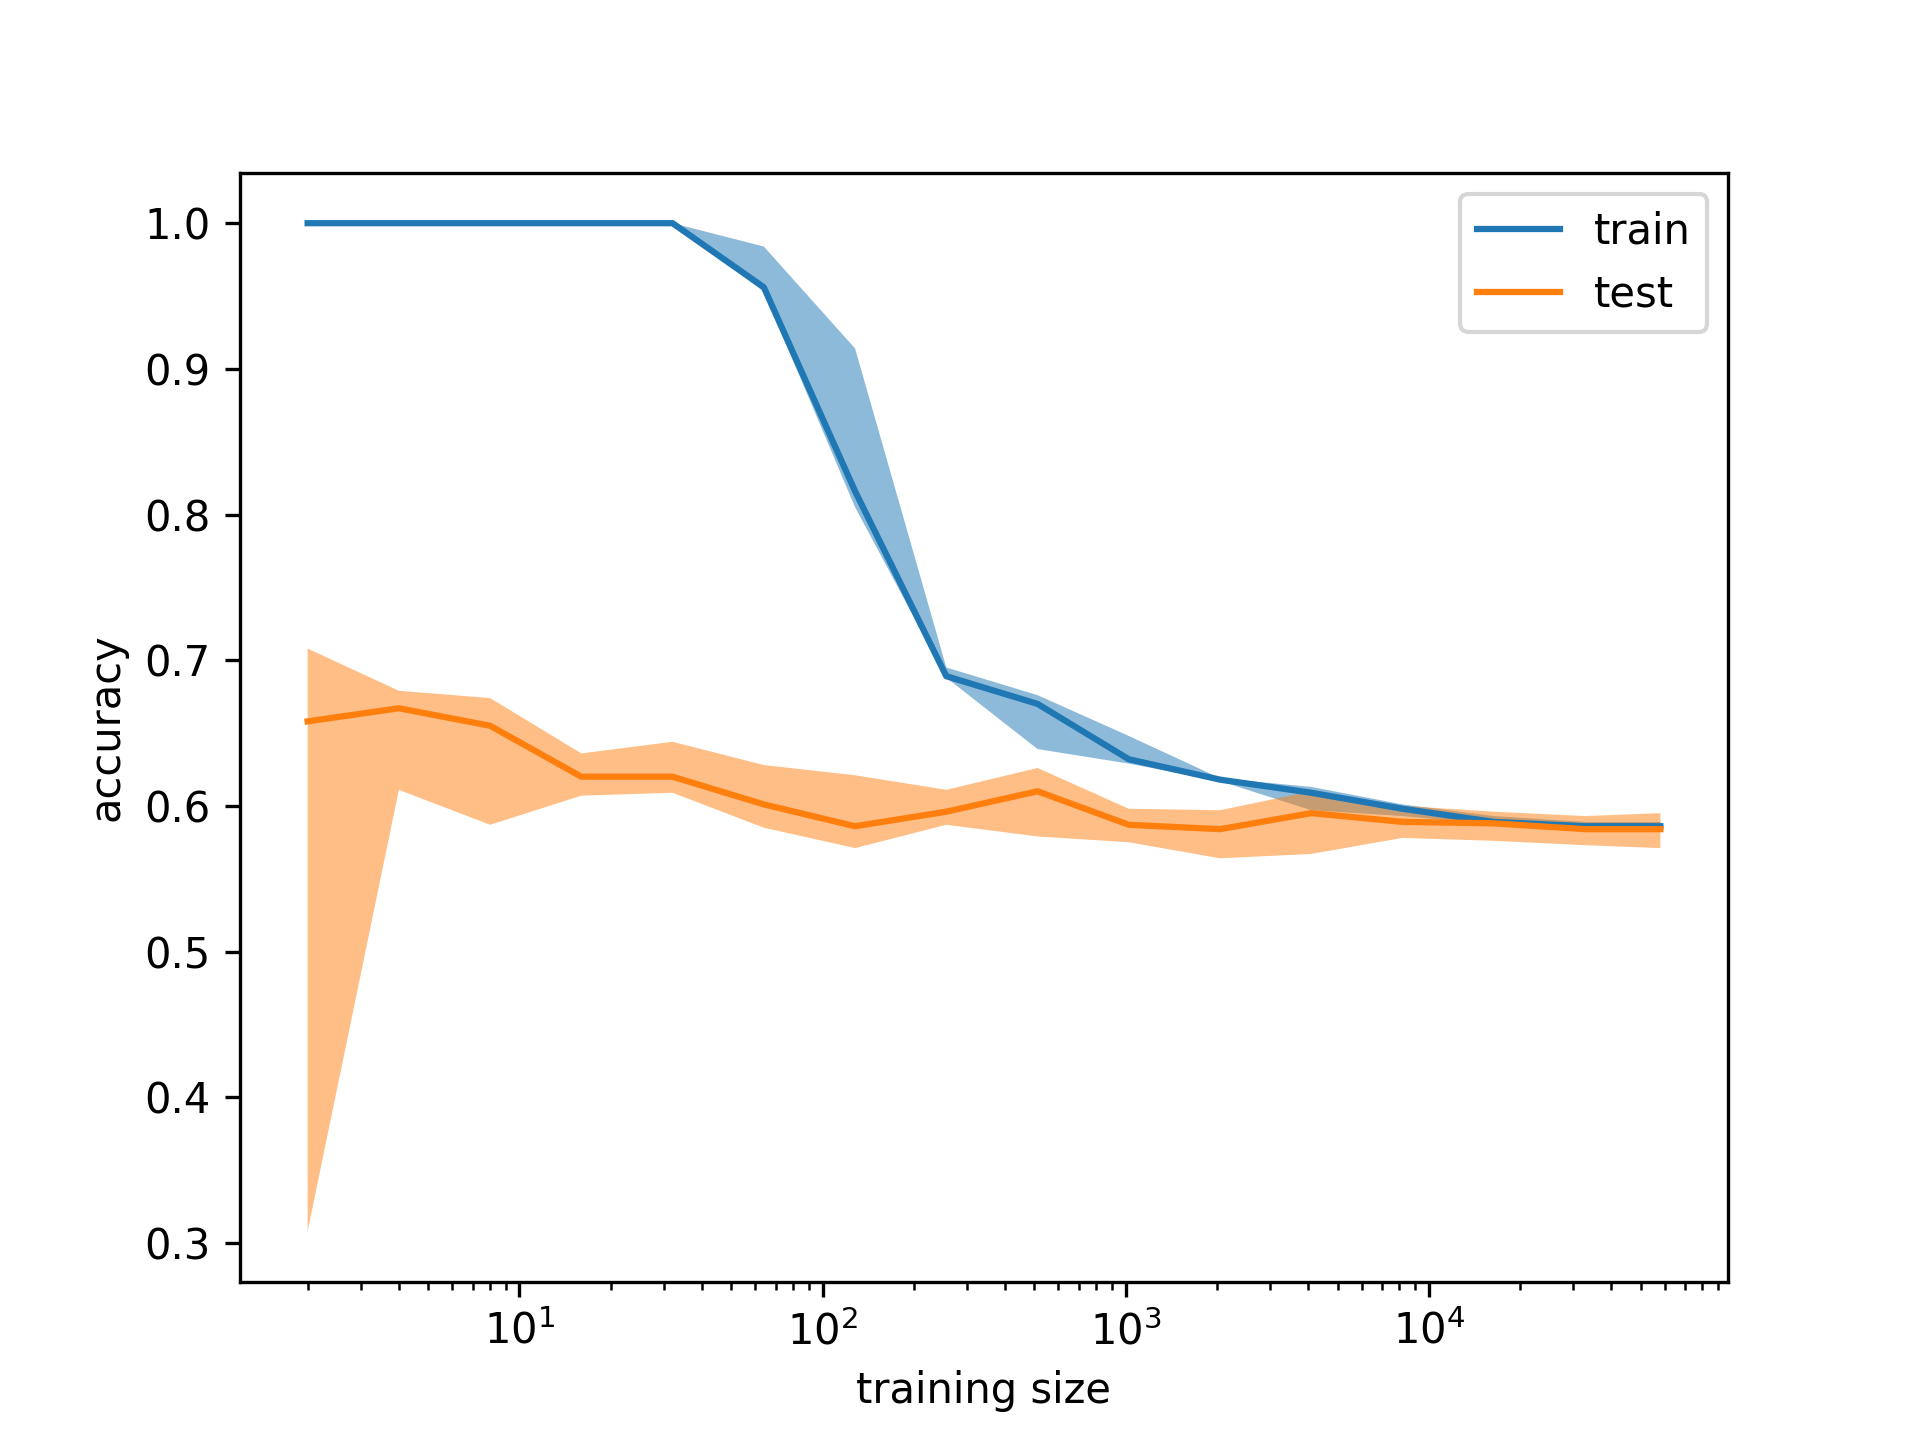
\includegraphics[width=130mm]{figures/l_curves_accuracy.png}
\caption{Dependency of accuracy on the training size}
\label{fig:l_curves_accuracy}
\end{figure}

\begin{figure}[h]\centering
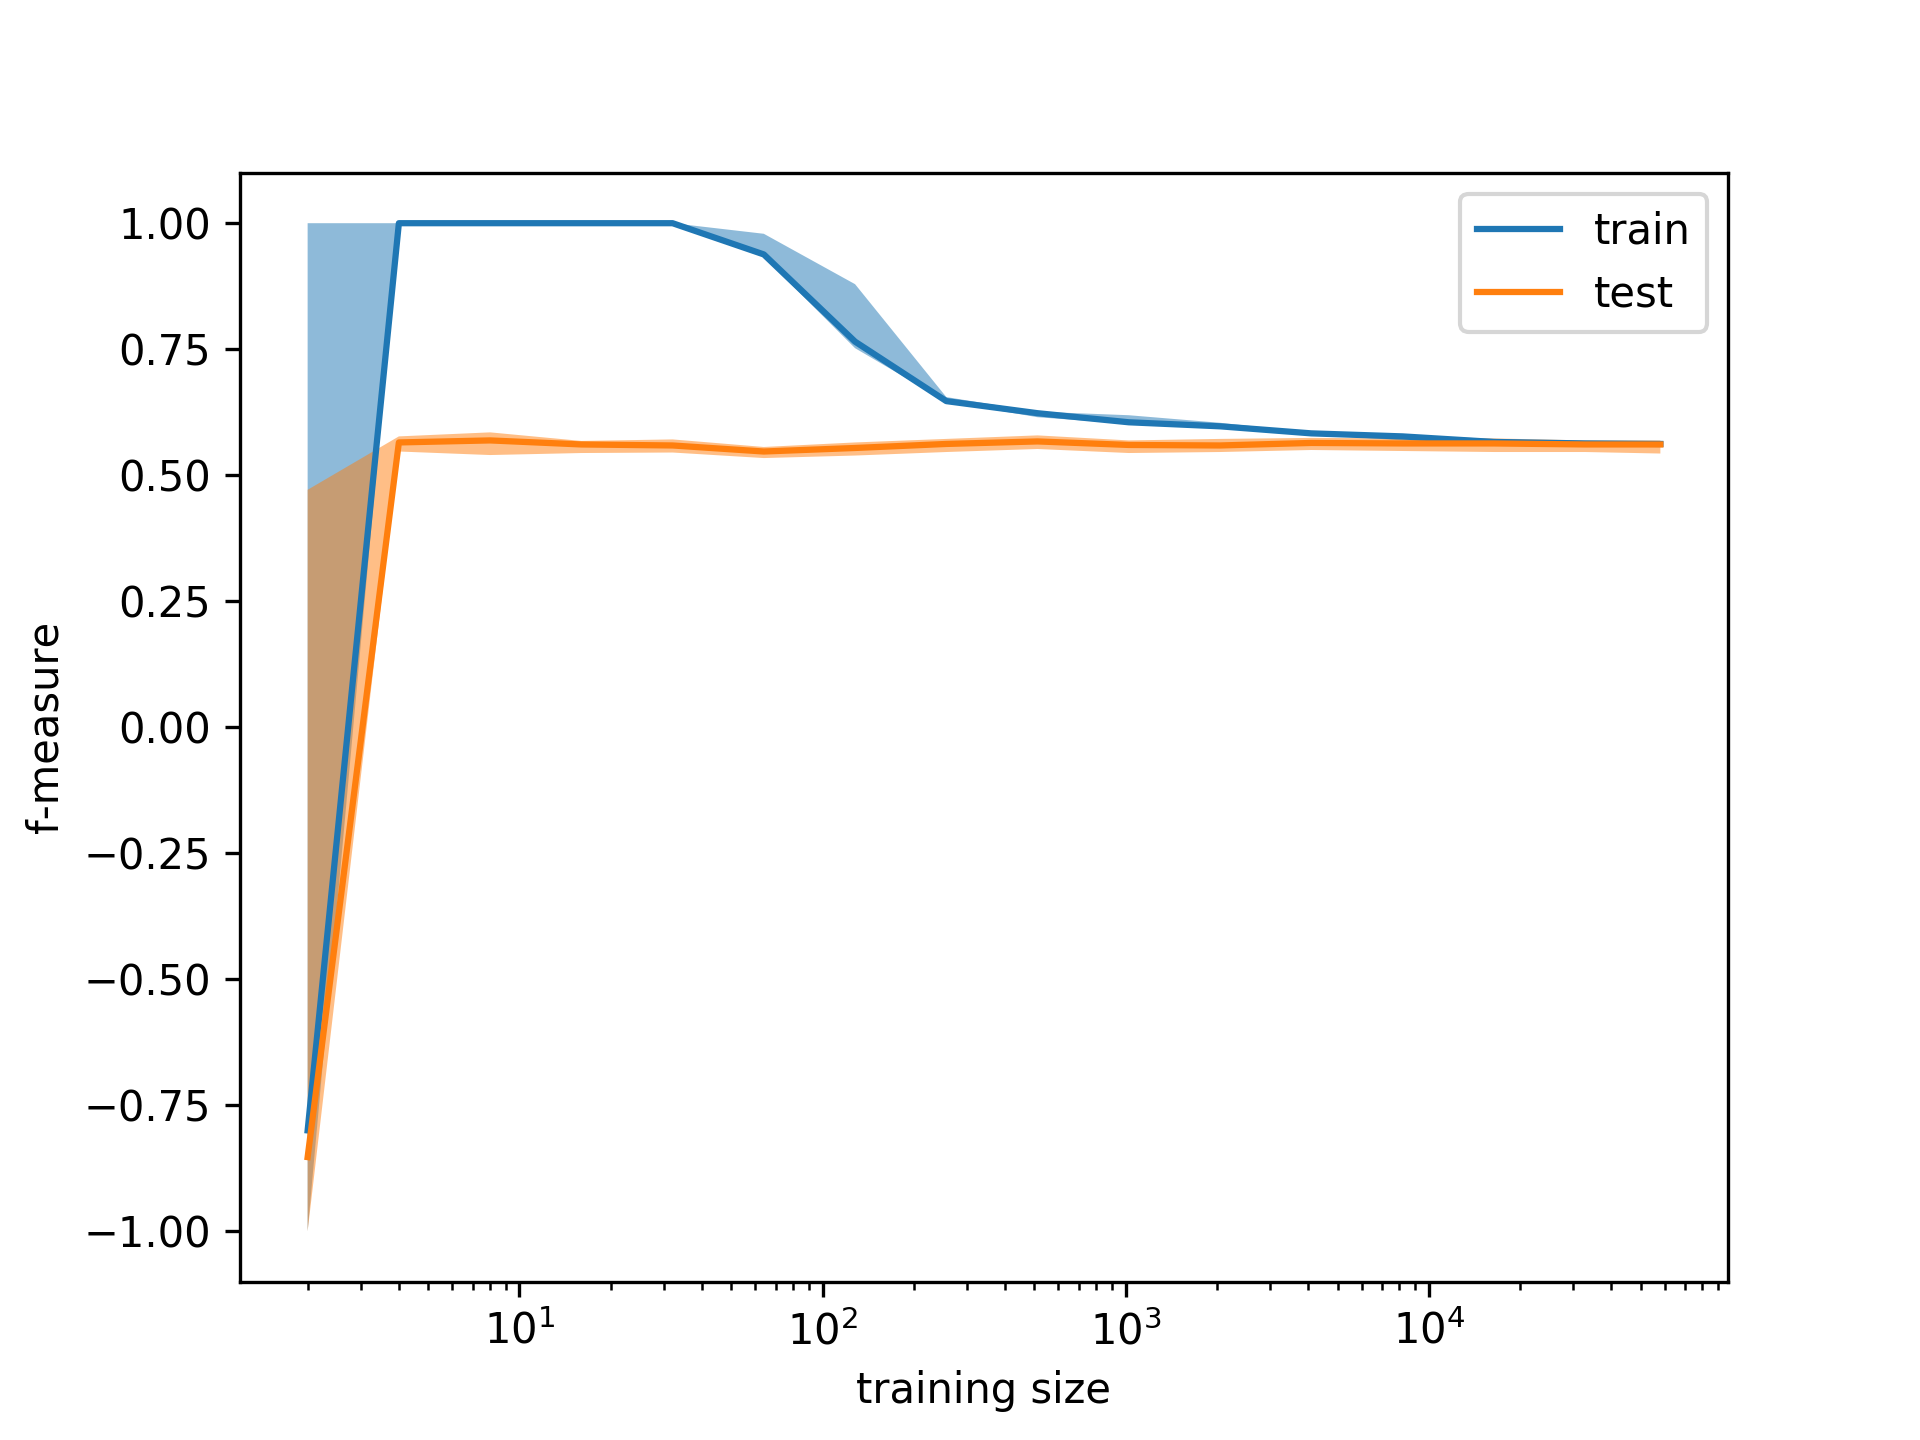
\includegraphics[width=130mm]{figures/l_curves_f_measure.png}
\caption{Dependency of f-measure on the training size}
\label{fig:l_curves_f_measure}
\end{figure}


We use processed data as described in \Cref{app:a}.
